\documentclass{article}

% if you need to pass options to natbib, use, e.g.:
%     \PassOptionsToPackage{numbers, compress}{natbib}
% before loading neurips_2020

% ready for submission
% \usepackage{neurips_2020}

% to compile a preprint version, e.g., for submission to arXiv, add add the
% [preprint] option:
%     \usepackage[preprint]{neurips_2020}

% to compile a camera-ready version, add the [final] option, e.g.:
    \usepackage[final]{neurips_2020}

% to avoid loading the natbib package, add option nonatbib:
    %  \usepackage[nonatbib]{neurips_2020}

\usepackage[utf8]{inputenc} % allow utf-8 input
\usepackage[T1]{fontenc}    % use 8-bit T1 fonts
\usepackage{hyperref}       % hyperlinks
\usepackage{url}            % simple URL typesetting
\usepackage{booktabs}       % professional-quality tables
\usepackage{amsfonts}       % blackboard math symbols
\usepackage{nicefrac}       % compact symbols for 1/2, etc.
\usepackage{microtype}      % microtypography
\usepackage{graphicx}
\usepackage{caption}

\title{Mask Wearing Classification}

% The \author macro works with any number of authors. There are two commands
% used to separate the names and addresses of multiple authors: \And and \AND.
%
% Using \And between authors leaves it to LaTeX to determine where to break the
% lines. Using \AND forces a line break at that point. So, if LaTeX puts 3 of 4
% authors names on the first line, and the last on the second line, try using
% \AND instead of \And before the third author name.

\author{%
  Chanwut Kittivorawong\thanks{\url{https://chanwutk.github.io}} \\
  Paul G. Allen School of Computer Science and Engineering\\
  University of Washington, Seattle\\
  Seattle, WA 98105 \\
  \texttt{chanwutk@cs.washington.edu} \\
  % examples of more authors
  \And
  Louis Maliyam \\
  Paul G. Allen School of Computer Science and Engineering\\
  University of Washington, Seattle\\
  Seattle, WA 98105 \\
  \texttt{maliyp@cs.washington.edu} \\
  % \AND
  % Coauthor \\
  % Affiliation \\
  % Address \\
  % \texttt{email} \\
  % \And
  % Coauthor \\
  % Affiliation \\
  % Address \\
  % \texttt{email} \\
  % \And
  % Coauthor \\
  % Affiliation \\
  % Address \\
  % \texttt{email} \\
}

\begin{document}

\maketitle

\begin{abstract}
As of the beginning of 2021, most restaurants, grocery stores, healthcare, and other public spaces are open.
However, people are required to wear a mask to enter those places.
In this paper, we create a camera application that determines whether a human face is wearing a mask.
The application classifies human faces using a convolutional neural network model.
This application can reduce the work of staff and increase higher protections for the sake of common benefits of everyone sharing the spaces.
\end{abstract}
\section{Introduction}
In the world of pandemics, it’s important to protect each other to slow down the spread of COVID-19.
According to Cheng et al. [1], wearing a mask is one of the most efficient ways to not pass on or to not receive COVID-19 from respiratory droplets.
Therefore, people are required to wear masks in many indoor facilities.
With this enforcement, each facility needs extra resources to monitor this activity.
For instance, staffs in a restaurant need to make sure that all customers wear masks.
We want to minimize the resources uses in this enforcement.
Therefore, we solved this problem by creating a camera application that detects whether a person is wearing a mask or not.
The application uses a convolutional neural network model for classification.
Then, we created an application that makes use of the neural network model by filming a person and detecting whether the person is wearing a mask or not, frame by frame and in real-time.
In the end, we evaluated our model performance, and we found that our model had a 92.16\% accuracy when testing with our dataset.
With some incorrect predictions, we wanted to find out what causes the model to incorrectly classify some images.
After the model was trained, we extracted the output of network layers from our model and compared the outputs from correctly classified images and incorrectly classified images.


\section{Datasets}

To train our model, we use Face Mask Detection Dataset owned by Gurav [2].
The datasets include 3,725 images of human faces wearing masks and 3,828 images of human faces without masks.
Then, we broke them down into two datasets–training dataset and test dataset. See Table~\ref{table:num-images-table}.

\begin{table}
  \caption{The number of images being used to train/test for each class}
  \label{table:num-images-table}
  \centering
  \begin{tabular}{lll}
    \toprule
    Classes       & Training Dataset & Testing Dataset \\
    \midrule
    with mask     & 3,354            & 371 \\
    without mask  & 3,446            & 382 \\
    \bottomrule
  \end{tabular}
\end{table}

\subsection{Data Preparation}
To ensure the consistency of input size, we resized every image into a square image with size 128 pixels by 128 pixels. In addition, we prepared the data before training by applying these transformations to our training data (Figure~\ref{fig:image-transformation}):
grayscale-filter, random rotation (-90 degrees to 90 degrees), random horizontal flip, and image normalization.
We applied the grayscale-filter because different cameras might have different color profiles.
The random rotation and random horizontal flip were applied so that our model did not overfit the training dataset.
The image normalization was applied so that the mean of each image was at the same point and distributed similarly.

\begin{figure}
  \caption{
    example of images that were transformed. We always resize the image to 128 pixels x pixels, apply grayscale and image normalization on them. We also perform random rotation and random horizontal flip on the images to generalize the model.
  }
  \label{fig:image-transformation}
  \centering
  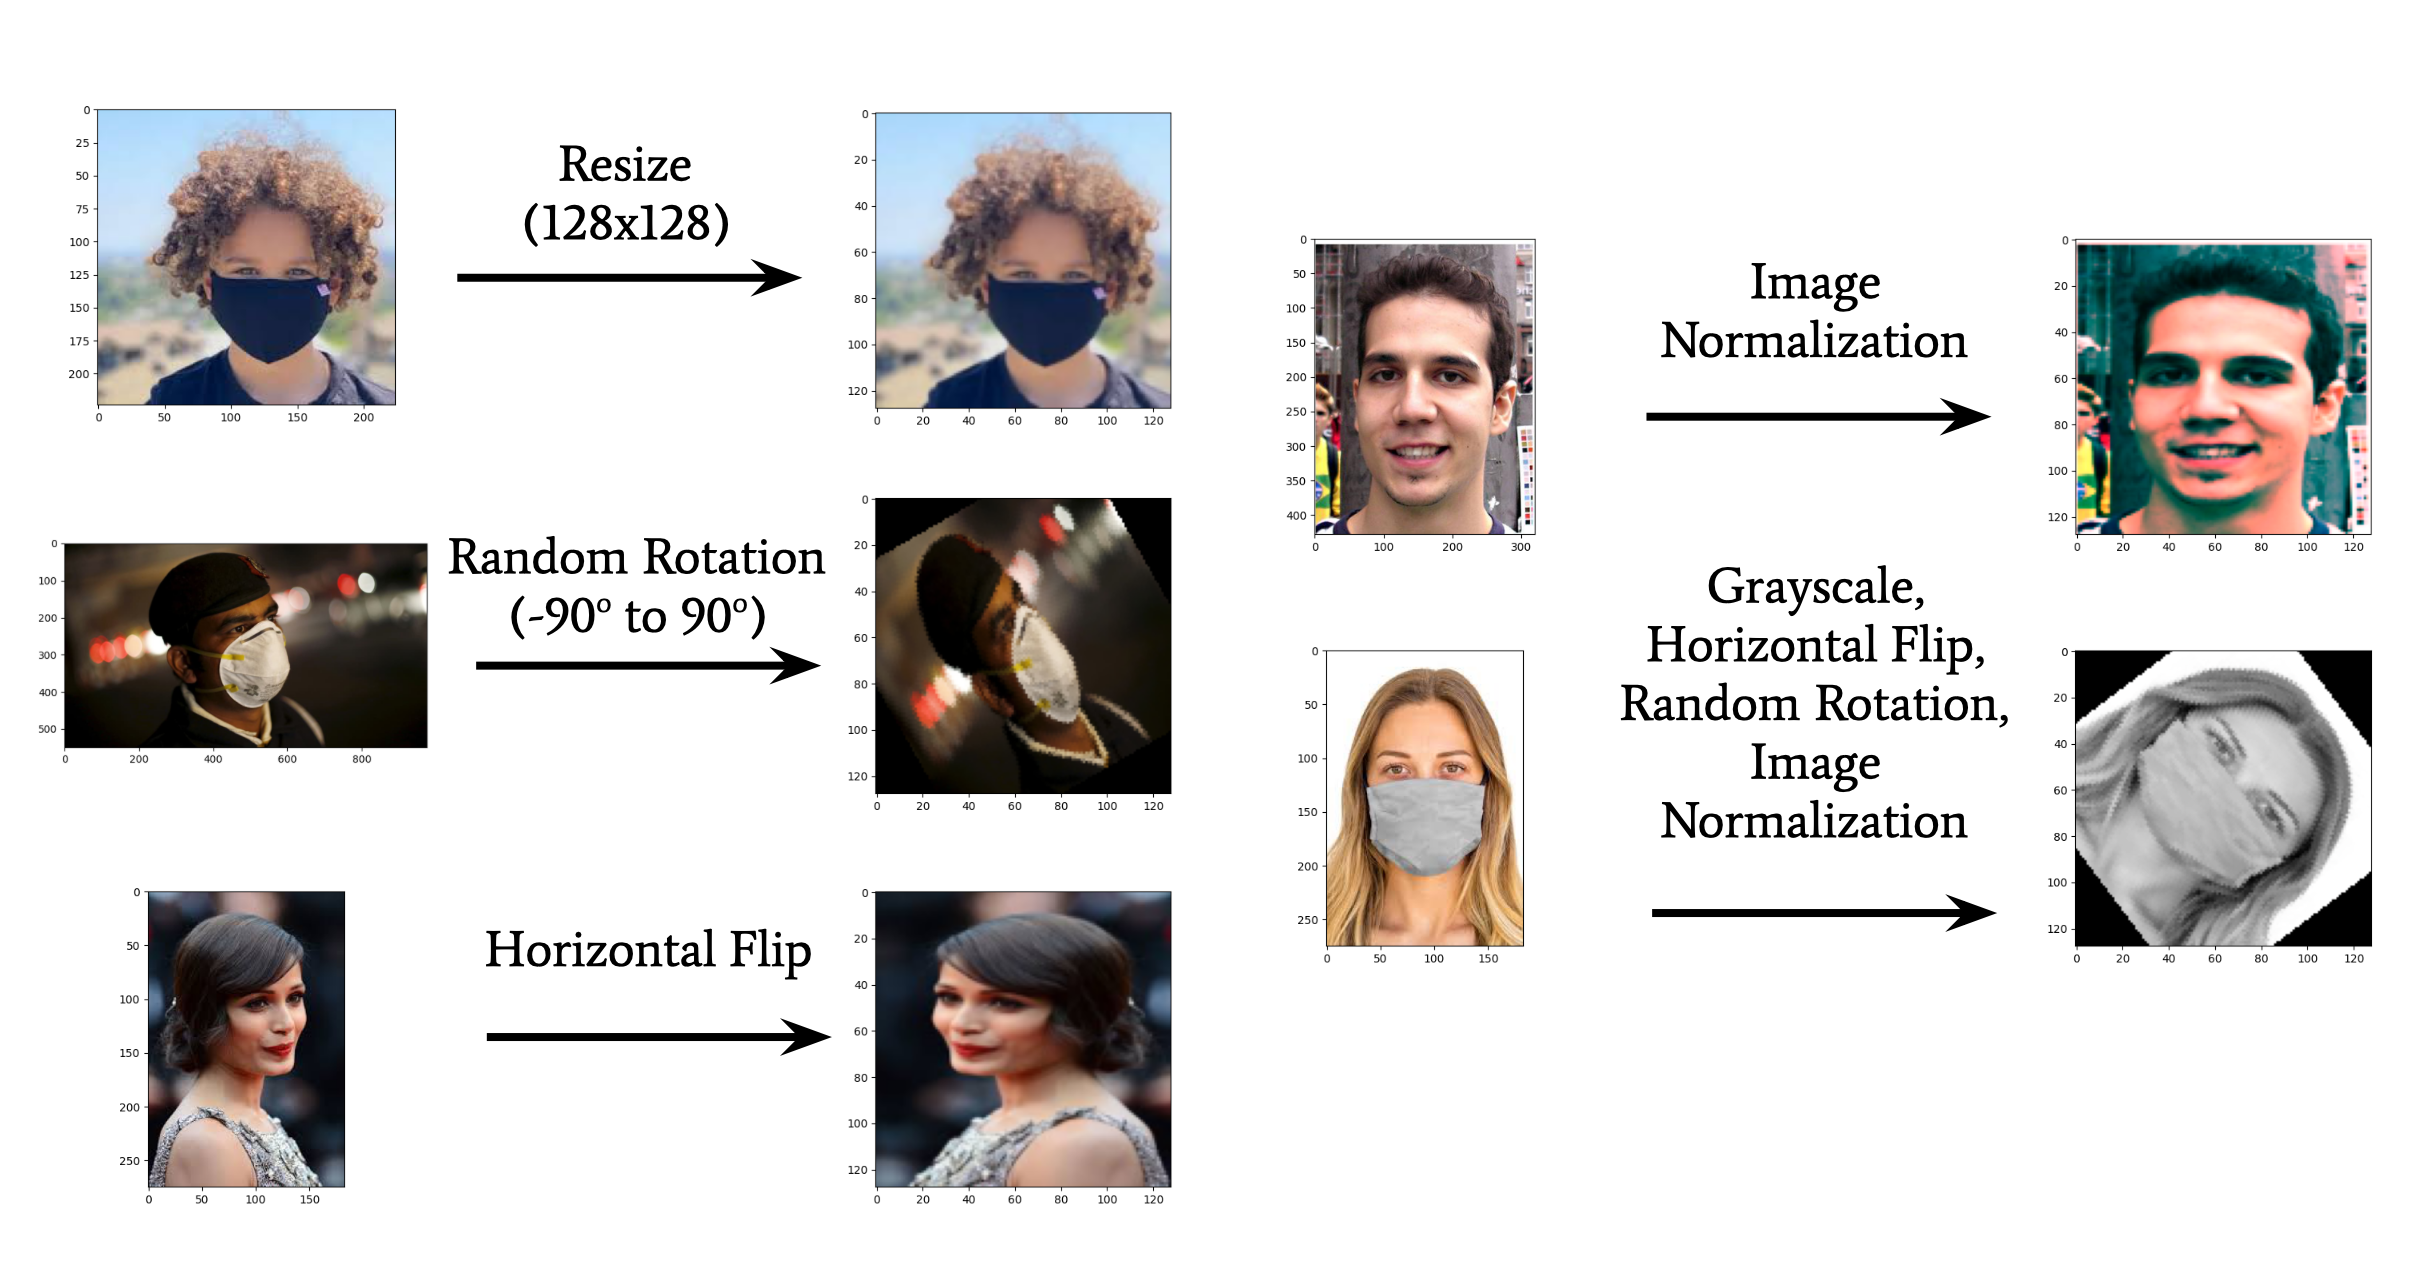
\includegraphics[height=150px]{figures/image-transformation.png}
\end{figure}
\section{Neural Network Model}

Since this problem is to classify images, we chose to use a deep neural network to efficiently and accurately solve the problem.
Specifically, we were using a convolutional neural network to detect whether people in the images were wearing masks.

\subsection{Model Structure}

The model receives a batch of grayscale images with the size of 128 pixels by 128 pixels as an input.
In order to predict the output, the model makes use of several hidden layers to come up with probability distribution (or predictions).

The model consists of three convolutional layers with a max-pooling layer after each of them.
We performed a batch normalization at the last convolutional neural network to make the model learns better. 
Moreover, we flattened the last max-pooling layer out to input into two fully connected layers which eventually predicted the output of the model.
The model can classify images into two classes–with mask and without mask. See Figure~\ref{fig:model-structure}.

\begin{figure}
  \caption{
    the architecture of the convolutional neural network,
    which consists of three convolutional layers with a max-pooling layer after each of them.
    The output from the last layer then being inputted into the last two fully connected layers which predict the final output.
  }
  \label{fig:model-structure}
  \centering
  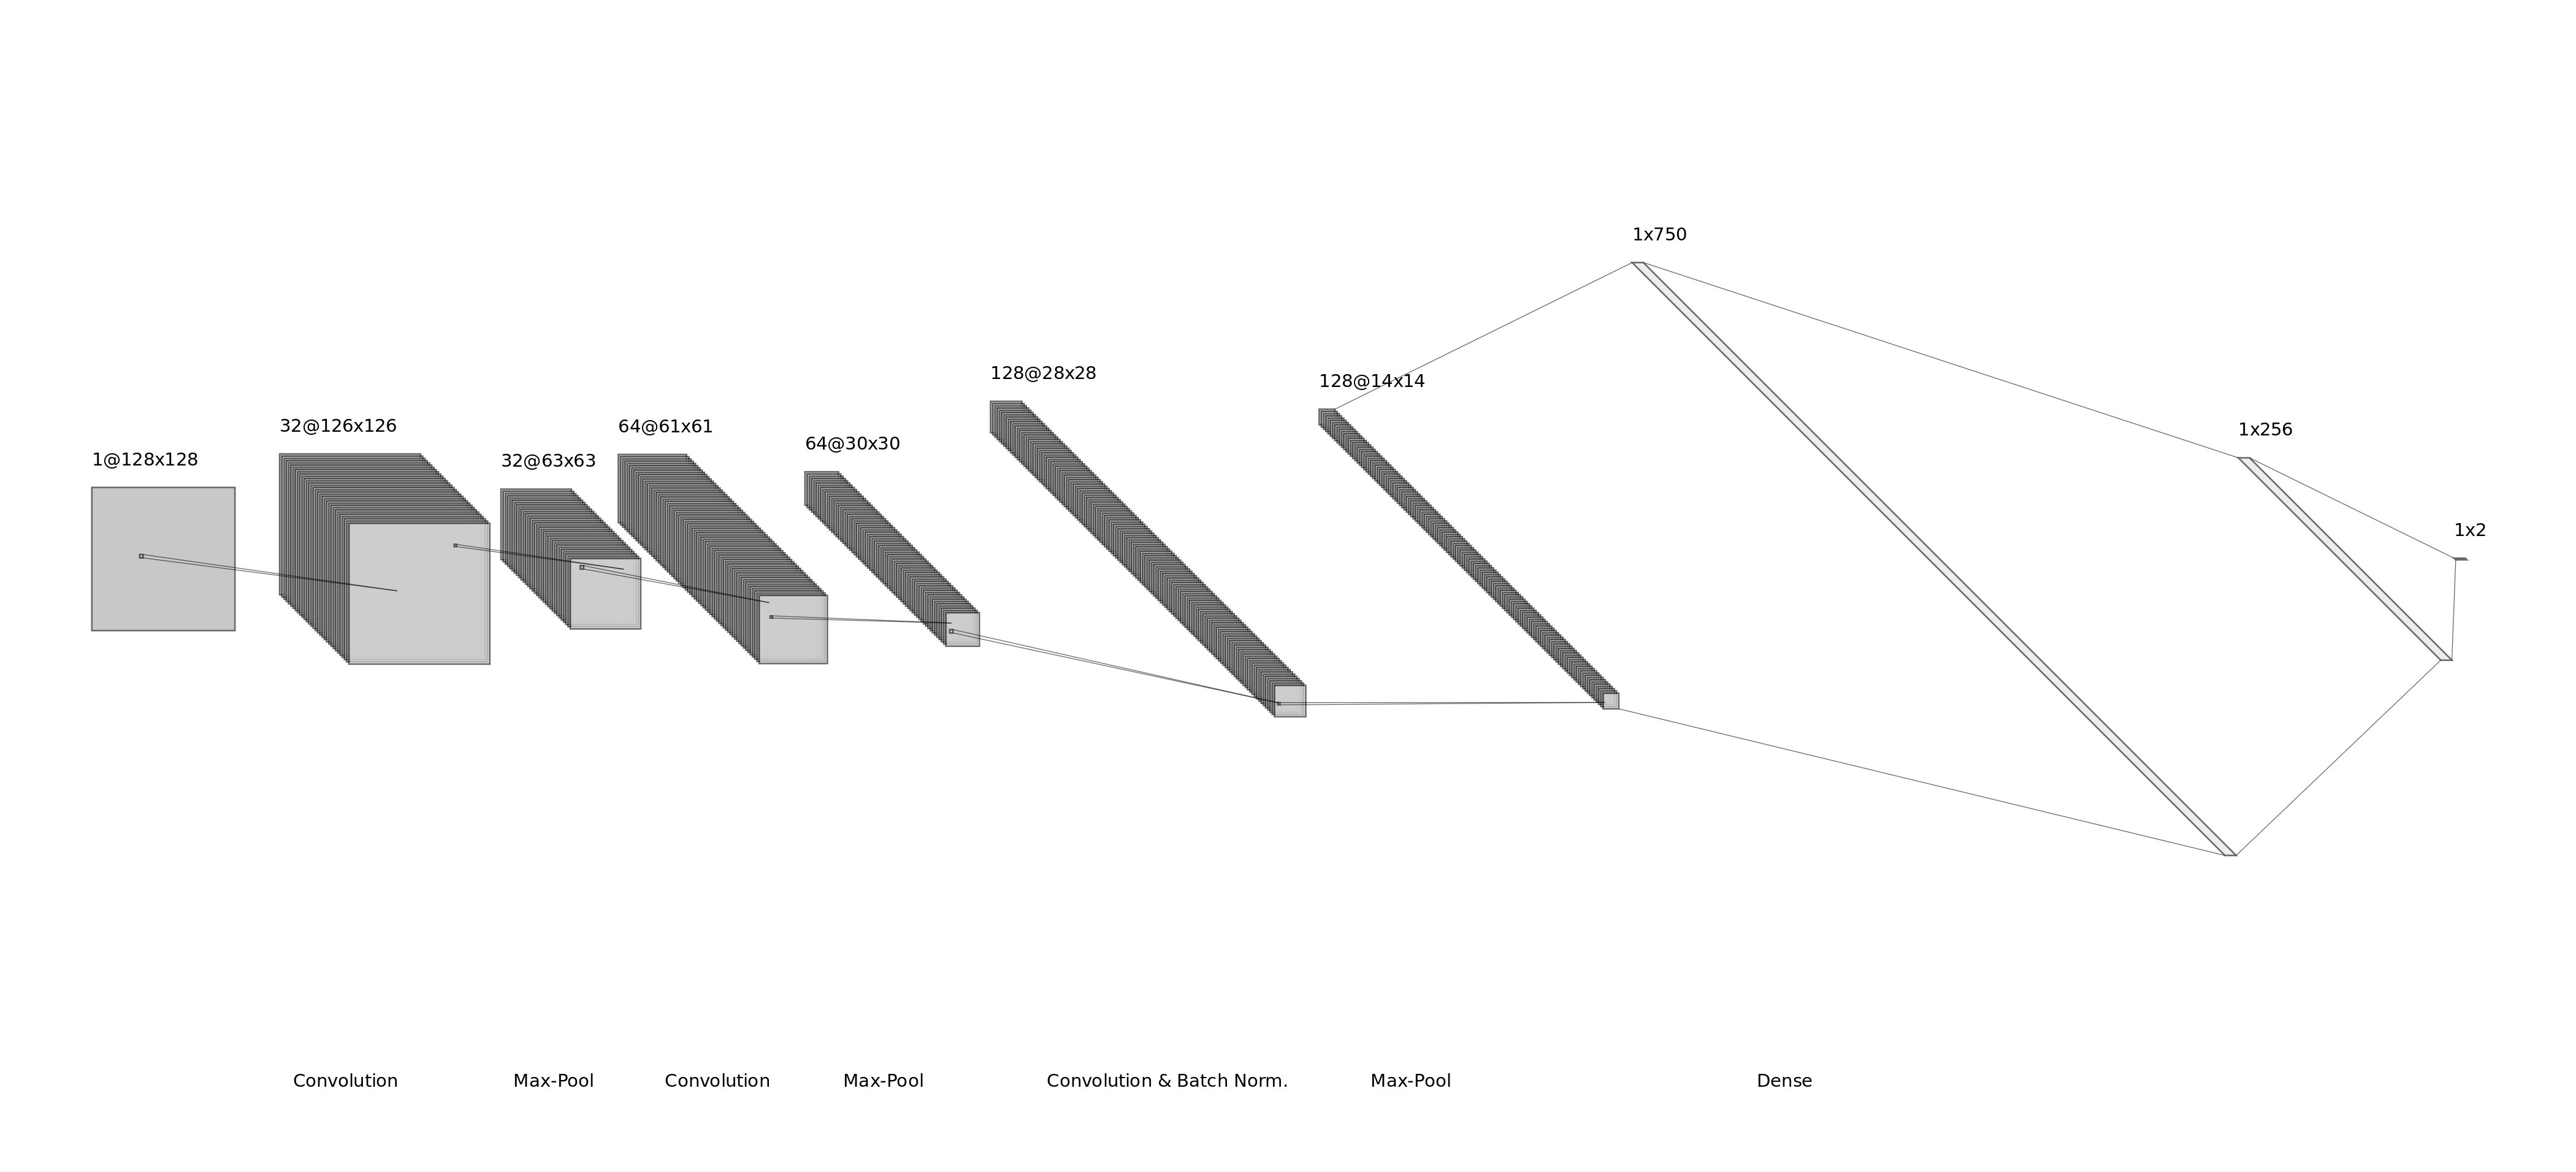
\includegraphics[width=400px]{figures/model-structure.jpg}
\end{figure}


\subsection{Loss Function and Optimizer}

We used softmax and cross-entropy as our loss functions.
We used softmax at the end of our prediction because the softmax function simulated the probability of an input image being one of the two classes.
And, we used the cross-entropy function at the end because we would like to amplify the loss value to penalize the model when it predicted incorrectly.
For an optimizer for our training, we used SGD because a model trained with SGD is less likely to overfit the dataset as it chooses data points at random.

\section{Results}

\subsection{Training and Model Performance}

We trained the model for 100 epochs using a learning rate of 0.01, a momentum of 0.9, and a weight decay of 0.0005. The final model yields 92.16\% accuracy on the test dataset.

\subsection{Prediction Examples}

Figure~\ref{fig:prediction-examples} shows some examples of images that were being tested and the output that the model predicted. The first row shows the images that are correctly predicted. The second row are images with people wearing masks, but our model falsely predicted that they were not wearing masks. The third row are images of people not wearing masks. However, our model incorrectly predicted that they were wearing masks.

Based on the examples here, we noticed that the images that were correctly predicted tend to have the following characteristics: (1) the human faces are large in the frame, (2) the face part and mask part are easily distinguishable, and (3) there is not much going on in the background.

On the opposite side, images that were incorrectly predicted might contain some of these characteristics: (1) there are variations of color and pattern on the masks, (2) images contain accessories and/or facial hair, which make the model misassociate them with the masks, and (3) the mask is not easily distinguishable from the face.

\begin{figure}
  \caption{
    examples of images that were used to test the model. The first row are images that the model predicted correctly. The second row and the third row are images that the model incorrectly predicted.
  }
  \label{fig:prediction-examples}
  \centering
  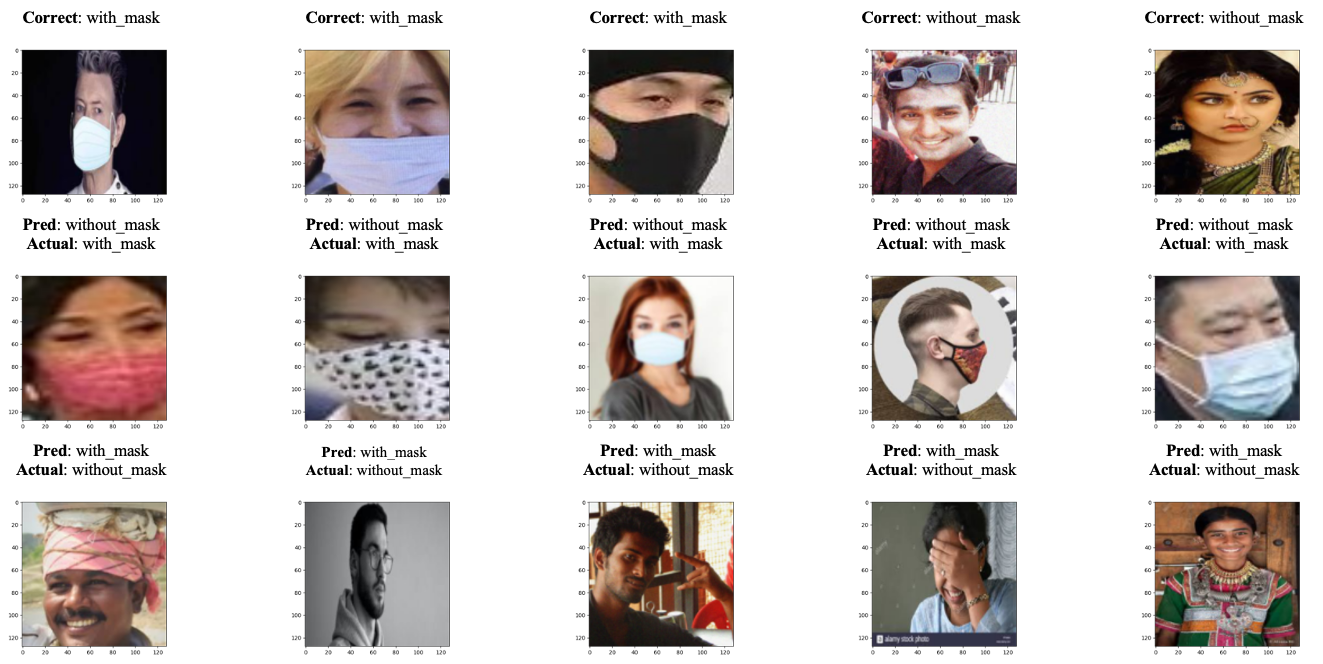
\includegraphics[width=300px]{figures/prediction-examples.png}
\end{figure}

\subsection{Output Layer Visualization}

As the model incorrectly predicted some images, we were curious about the cause of these incorrect predictions.
So, we extracted and visualized the output of the first ReLU layer to see the pattern of what pixels were activated.
In other words, we wanted to know what features our model captured from the images.
Starting from a correctly predicted image (Figure~\ref{fig:output-correct}), we can see that some channels either activate the face part or the mask part.
So, the model can distinguish between the two parts.
Furthermore, we can see that our model can capture the eyes of the humans in the images.
On the other hand, our model cannot capture some of these features in the incorrectly classified images.
In the first incorrectly classified example (Figure~\ref{fig:output-incorrect-1}), our model could not find the clear boundaries between face and mask.
In the second incorrectly classified example (Figure~\ref{fig:output-incorrect-2}), our model could not capture the eyes of the humans in the image.
In the third incorrectly classified example (Figure~\ref{fig:output-incorrect-3}), our model activated the parts of the image that were not the human face.


\subsection{Camera Application}
Our camera application captures video of human faces.
It then processes the video in real-time, frame by frame, by classifying if a human in the frame is wearing a mask or not.
Our camera application does well when the human face is close to the camera (Figure~\ref{fig:camera-correct}).
However, when the human face is far away or when the background of the video has too many objects (Figure~\ref{fig:camera-incorrect}), our model becomes inaccurate.
One future improvement in response to this problem is that we would like to cut out only the human face part of the image before classifying it.
With this improvement, the background of the video becomes irrelevant and will improve the accuracy of our application.

% \section{Conclusion}

Content here...
\section*{Broader Impact}

In this paper, we created a camera application that classifies human faces if they are wearing masks or not.
This application can make a big impact in the world of pandemics where people are required to wear masks inside indoor facilities.
With this application, these facilities can reduce the number of staff to monitor this enforcement and use machines, instead.
However, there is a downside to this application, as well.
This camera application could raise concerns in privacy as it records human faces.
In the real-world use, we would need to inform the visitors of these indoor facilities that our application only uses but not keep the video of anyone.
We also explored the problem behind the inaccuracy of our application by visualizing the layer outputs of our model.
We found that many incorrect classifications come from the fact that these images have many objects in the background and confuse our model.
In future work, we would like to improve our application by adding another neural network that detects faces.
Then, we can crop only the face part to be classified using our current model.

\begin{ack}
We thank all the UW CSE 573 staffs for their helps in this class.
\end{ack}
\section*{References}

% References follow the acknowledgments. Use unnumbered first-level heading for
% the references. Any choice of citation style is acceptable as long as you are
% consistent. It is permissible to reduce the font size to \verb+small+ (9 point)
% when listing the references.
% {\bf Note that the Reference section does not count towards the eight pages of content that are allowed.}
\medskip

\small

[1] Cheng, V., Wong, S., Chuang, V., So, S., Chen, J., Sridhar, S., To, K., Chan, J., Hung, I., Ho, P. \ \& Yuen, K.\ (2020) {\it The role of community-wide wearing of face mask for control of coronavirus disease 2019 (COVID-19) epidemic due to SARS-CoV-2} \url{https://www.sciencedirect.com/science/article/abs/pii/S0163445320302358?casa_token=BI_okioGo04AAAAA:FB5PL1IYJ3KPUCDHp83V6BywFXXEnifn5VSOTYZ9koedSRdJLWJ6iBJn69nXXG57GR1mTiyL-OY}

[2] Gurav, O. \ (2020) {\it Face Mask Detection Dataset}. \url{https://www.kaggle.com/omkargurav/face-mask-dataset/metadata}

% [1] Alexander, J.A.\ \& Mozer, M.C.\ (1995) Template-based algorithms for
% connectionist rule extraction. In G.\ Tesauro, D.S.\ Touretzky and T.K.\ Leen
% (eds.), {\it Advances in Neural Information Processing Systems 7},
% pp.\ 609--616. Cambridge, MA: MIT Press.

% [2] Bower, J.M.\ \& Beeman, D.\ (1995) {\it The Book of GENESIS: Exploring
%   Realistic Neural Models with the GEneral NEural SImulation System.}  New York:
% TELOS/Springer--Verlag.

% [3] Hasselmo, M.E., Schnell, E.\ \& Barkai, E.\ (1995) Dynamics of learning and
% recall at excitatory recurrent synapses and cholinergic modulation in rat
% hippocampal region CA3. {\it Journal of Neuroscience} {\bf 15}(7):5249-5262.
\section*{Appendix}

\begin{center}
  \captionof{figure}{Output tensor of the first ReLU layer of a correctly classified image}
  \label{fig:output-correct}
  \centering
  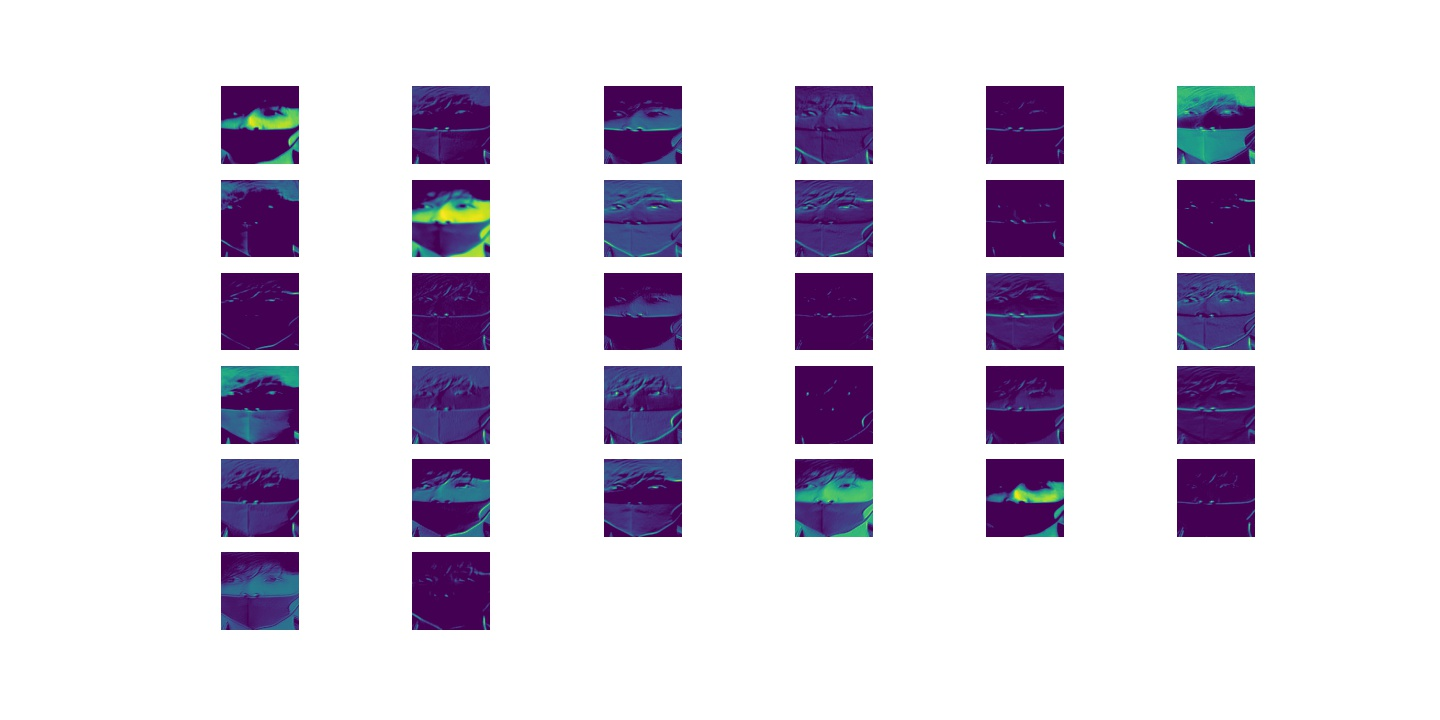
\includegraphics[width=300px]{figures/correct_first_layer_0.jpg}
\end{center}

\begin{center}
  \captionof{figure}{Output tensor of the first ReLU layer of an incorrectly classified image}
  \label{fig:output-incorrect-1}
  \centering
  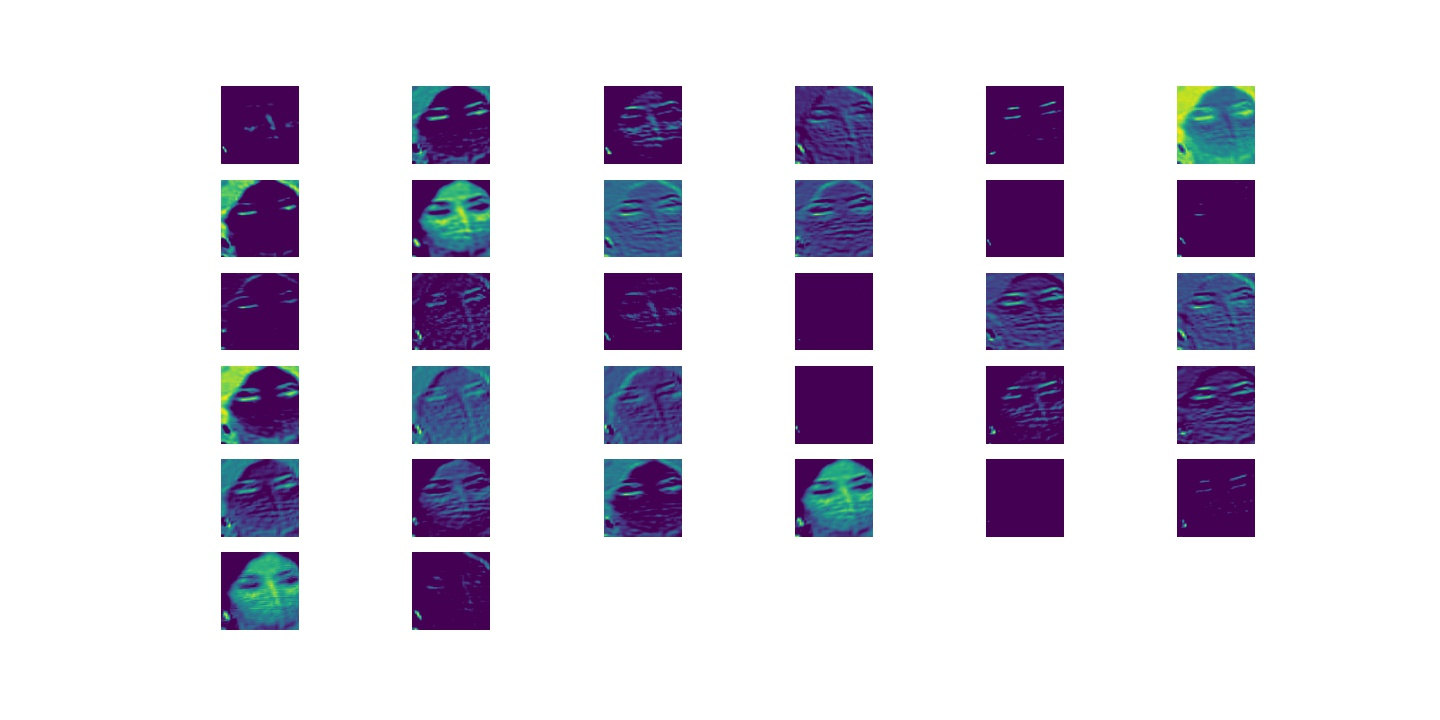
\includegraphics[width=300px]{figures/incorrect_first_layer_0.jpg}
\end{center}

\begin{center}
  \captionof{figure}{Output tensor of the first ReLU layer of an incorrectly classified image}
  \label{fig:output-incorrect-2}
  \centering
  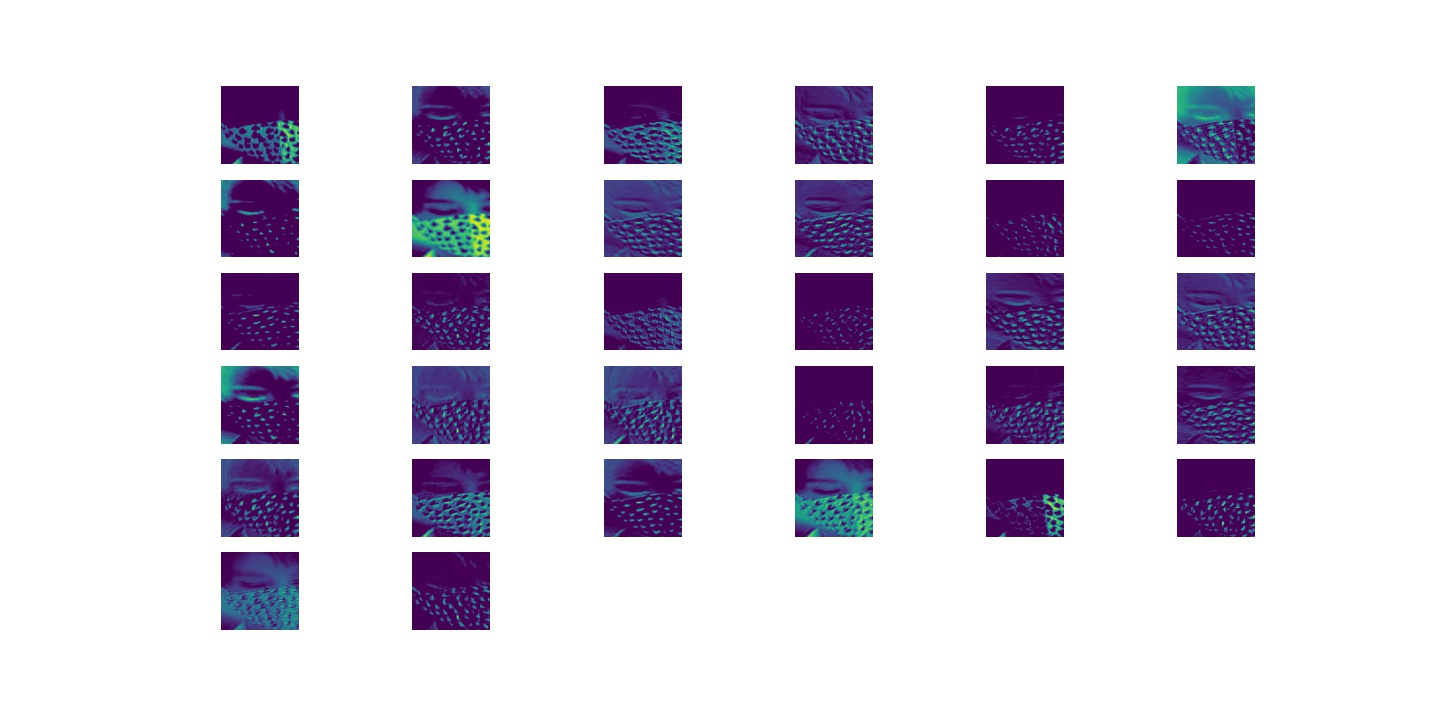
\includegraphics[width=300px]{figures/incorrect_first_layer_2.jpg}
\end{center}

\newpage

\begin{center}
  \captionof{figure}{Output tensor of the first ReLU layer of an incorrectly classified image}
  \label{fig:output-incorrect-3}
  \centering
  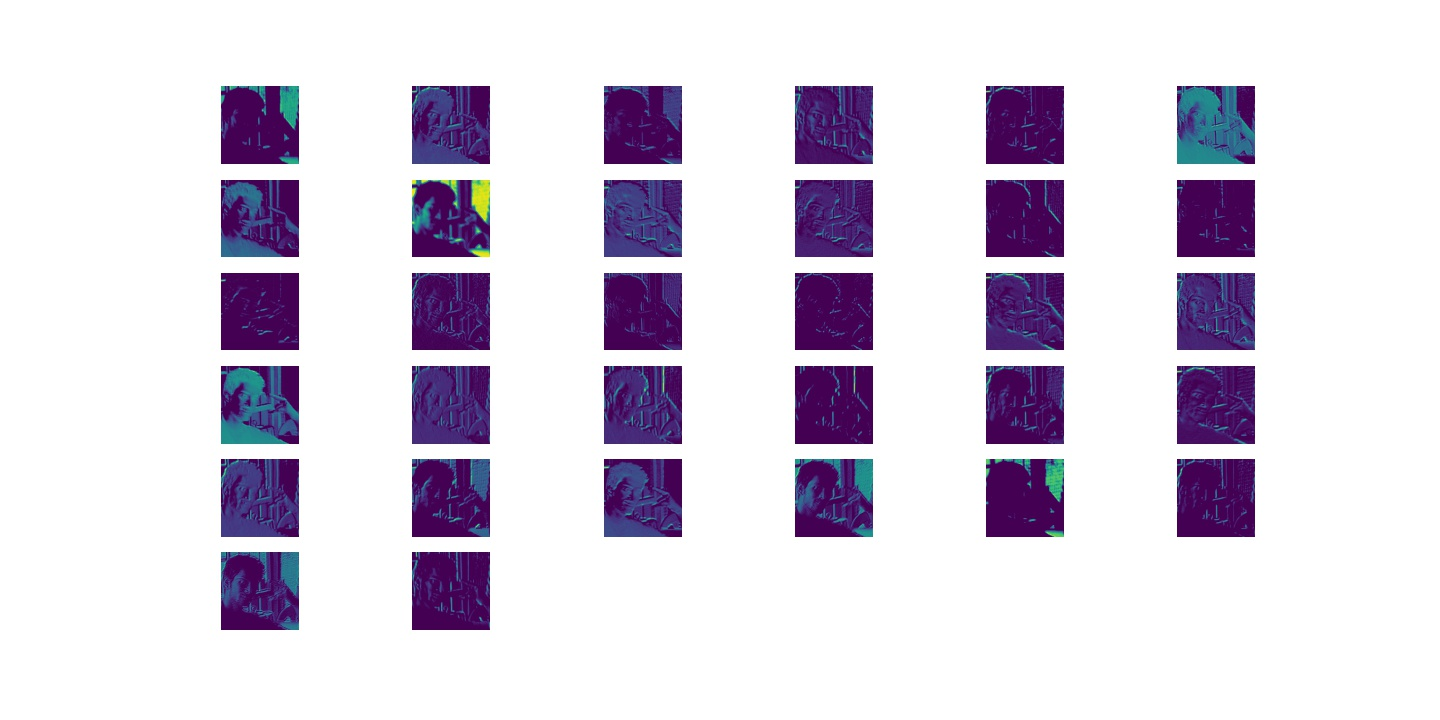
\includegraphics[width=300px]{figures/incorrect_first_layer_16.jpg}
\end{center}

\begin{center}
  \captionof{figure}{Camera application when correctly classified a face}
  \label{fig:camera-correct}
  \centering
  \includegraphics[width=300px]{figures/camera_correct.png}
\end{center}

\begin{center}
  \captionof{figure}{Camera application when incorrectly classified a face}
  \label{fig:camera-incorrect}
  \centering
  \includegraphics[width=300px]{figures/camera_incorrect.png}
\end{center}

% -------------------------------------------------------------
% TODO: remove from here -------------------------------------
% -------------------------------------------------------------

% \section{Submission of papers to NeurIPS 2020}

% NeurIPS requires electronic submissions.  The electronic submission site is
% \begin{center}
%   \url{https://cmt3.research.microsoft.com/NeurIPS2020/}
% \end{center}

% Please read the instructions below carefully and follow them faithfully.

% \subsection{Style}

% Papers to be submitted to NeurIPS 2020 must be prepared according to the
% instructions presented here. Papers may only be up to eight pages long,
% including figures. Additional pages \emph{containing only a section on the broader impact, acknowledgments and/or cited references} are allowed. Papers that exceed eight pages of content will not be reviewed, or in any other way considered for
% presentation at the conference.

% The margins in 2020 are the same as those in 2007, which allow for $\sim$$15\%$
% more words in the paper compared to earlier years.

% Authors are required to use the NeurIPS \LaTeX{} style files obtainable at the
% NeurIPS website as indicated below. Please make sure you use the current files
% and not previous versions. Tweaking the style files may be grounds for
% rejection.

% \subsection{Retrieval of style files}

% The style files for NeurIPS and other conference information are available on
% the World Wide Web at
% \begin{center}
%   \url{http://www.neurips.cc/}
% \end{center}
% The file \verb+neurips_2020.pdf+ contains these instructions and illustrates the
% various formatting requirements your NeurIPS paper must satisfy.

% The only supported style file for NeurIPS 2020 is \verb+neurips_2020.sty+,
% rewritten for \LaTeXe{}.  \textbf{Previous style files for \LaTeX{} 2.09,
%   Microsoft Word, and RTF are no longer supported!}

% The \LaTeX{} style file contains three optional arguments: \verb+final+, which
% creates a camera-ready copy, \verb+preprint+, which creates a preprint for
% submission to, e.g., arXiv, and \verb+nonatbib+, which will not load the
% \verb+natbib+ package for you in case of package clash.

% \paragraph{Preprint option}
% If you wish to post a preprint of your work online, e.g., on arXiv, using the
% NeurIPS style, please use the \verb+preprint+ option. This will create a
% nonanonymized version of your work with the text ``Preprint. Work in progress.''
% in the footer. This version may be distributed as you see fit. Please \textbf{do
%   not} use the \verb+final+ option, which should \textbf{only} be used for
% papers accepted to NeurIPS.

% At submission time, please omit the \verb+final+ and \verb+preprint+
% options. This will anonymize your submission and add line numbers to aid
% review. Please do \emph{not} refer to these line numbers in your paper as they
% will be removed during generation of camera-ready copies.

% The file \verb+neurips_2020.tex+ may be used as a ``shell'' for writing your
% paper. All you have to do is replace the author, title, abstract, and text of
% the paper with your own.

% The formatting instructions contained in these style files are summarized in
% Sections \ref{gen_inst}, \ref{headings}, and \ref{others} below.

% \section{General formatting instructions}
% \label{gen_inst}

% The text must be confined within a rectangle 5.5~inches (33~picas) wide and
% 9~inches (54~picas) long. The left margin is 1.5~inch (9~picas).  Use 10~point
% type with a vertical spacing (leading) of 11~points.  Times New Roman is the
% preferred typeface throughout, and will be selected for you by default.
% Paragraphs are separated by \nicefrac{1}{2}~line space (5.5 points), with no
% indentation.

% The paper title should be 17~point, initial caps/lower case, bold, centered
% between two horizontal rules. The top rule should be 4~points thick and the
% bottom rule should be 1~point thick. Allow \nicefrac{1}{4}~inch space above and
% below the title to rules. All pages should start at 1~inch (6~picas) from the
% top of the page.

% For the final version, authors' names are set in boldface, and each name is
% centered above the corresponding address. The lead author's name is to be listed
% first (left-most), and the co-authors' names (if different address) are set to
% follow. If there is only one co-author, list both author and co-author side by
% side.

% Please pay special attention to the instructions in Section \ref{others}
% regarding figures, tables, acknowledgments, and references.

% \section{Headings: first level}
% \label{headings}

% All headings should be lower case (except for first word and proper nouns),
% flush left, and bold.

% First-level headings should be in 12-point type.

% \subsection{Headings: second level}

% Second-level headings should be in 10-point type.

% \subsubsection{Headings: third level}

% Third-level headings should be in 10-point type.

% \paragraph{Paragraphs}

% There is also a \verb+\paragraph+ command available, which sets the heading in
% bold, flush left, and inline with the text, with the heading followed by 1\,em
% of space.

% \section{Citations, figures, tables, references}
% \label{others}

% These instructions apply to everyone.

% \subsection{Citations within the text}

% The \verb+natbib+ package will be loaded for you by default.  Citations may be
% author/year or numeric, as long as you maintain internal consistency.  As to the
% format of the references themselves, any style is acceptable as long as it is
% used consistently.

% The documentation for \verb+natbib+ may be found at
% \begin{center}
%   \url{http://mirrors.ctan.org/macros/latex/contrib/natbib/natnotes.pdf}
% \end{center}
% Of note is the command \verb+\citet+, which produces citations appropriate for
% use in inline text.  For example,
% \begin{verbatim}
%   \citet{hasselmo} investigated\dots
% \end{verbatim}
% produces
% \begin{quote}
%   Hasselmo, et al.\ (1995) investigated\dots
% \end{quote}

% If you wish to load the \verb+natbib+ package with options, you may add the
% following before loading the \verb+neurips_2020+ package:
% \begin{verbatim}
%   \PassOptionsToPackage{options}{natbib}
% \end{verbatim}

% If \verb+natbib+ clashes with another package you load, you can add the optional
% argument \verb+nonatbib+ when loading the style file:
% \begin{verbatim}
%   \usepackage[nonatbib]{neurips_2020}
% \end{verbatim}

% As submission is double blind, refer to your own published work in the third
% person. That is, use ``In the previous work of Jones et al.\ [4],'' not ``In our
% previous work [4].'' If you cite your other papers that are not widely available
% (e.g., a journal paper under review), use anonymous author names in the
% citation, e.g., an author of the form ``A.\ Anonymous.''

% \subsection{Footnotes}

% Footnotes should be used sparingly.  If you do require a footnote, indicate
% footnotes with a number\footnote{Sample of the first footnote.} in the
% text. Place the footnotes at the bottom of the page on which they appear.
% Precede the footnote with a horizontal rule of 2~inches (12~picas).

% Note that footnotes are properly typeset \emph{after} punctuation
% marks.\footnote{As in this example.}

% \subsection{Figures}

% \begin{figure}
%   \centering
%   \fbox{\rule[-.5cm]{0cm}{4cm} \rule[-.5cm]{4cm}{0cm}}
%   \caption{Sample figure caption.}
% \end{figure}

% All artwork must be neat, clean, and legible. Lines should be dark enough for
% purposes of reproduction. The figure number and caption always appear after the
% figure. Place one line space before the figure caption and one line space after
% the figure. The figure caption should be lower case (except for first word and
% proper nouns); figures are numbered consecutively.

% You may use color figures.  However, it is best for the figure captions and the
% paper body to be legible if the paper is printed in either black/white or in
% color.

% \subsection{Tables}

% All tables must be centered, neat, clean and legible.  The table number and
% title always appear before the table.  See Table~\ref{sample-table}.

% Place one line space before the table title, one line space after the
% table title, and one line space after the table. The table title must
% be lower case (except for first word and proper nouns); tables are
% numbered consecutively.

% Note that publication-quality tables \emph{do not contain vertical rules.} We
% strongly suggest the use of the \verb+booktabs+ package, which allows for
% typesetting high-quality, professional tables:
% \begin{center}
%   \url{https://www.ctan.org/pkg/booktabs}
% \end{center}
% This package was used to typeset Table~\ref{sample-table}.

% \begin{table}
%   \caption{Sample table title}
%   \label{sample-table}
%   \centering
%   \begin{tabular}{lll}
%     \toprule
%     \multicolumn{2}{c}{Part}                   \\
%     \cmidrule(r){1-2}
%     Name     & Description     & Size ($\mu$m) \\
%     \midrule
%     Dendrite & Input terminal  & $\sim$100     \\
%     Axon     & Output terminal & $\sim$10      \\
%     Soma     & Cell body       & up to $10^6$  \\
%     \bottomrule
%   \end{tabular}
% \end{table}

% \section{Final instructions}

% Do not change any aspects of the formatting parameters in the style files.  In
% particular, do not modify the width or length of the rectangle the text should
% fit into, and do not change font sizes (except perhaps in the
% \textbf{References} section; see below). Please note that pages should be
% numbered.

% \section{Preparing PDF files}

% Please prepare submission files with paper size ``US Letter,'' and not, for
% example, ``A4.''

% Fonts were the main cause of problems in the past years. Your PDF file must only
% contain Type 1 or Embedded TrueType fonts. Here are a few instructions to
% achieve this.

% \begin{itemize}

% \item You should directly generate PDF files using \verb+pdflatex+.

% \item You can check which fonts a PDF files uses.  In Acrobat Reader, select the
%   menu Files$>$Document Properties$>$Fonts and select Show All Fonts. You can
%   also use the program \verb+pdffonts+ which comes with \verb+xpdf+ and is
%   available out-of-the-box on most Linux machines.

% \item The IEEE has recommendations for generating PDF files whose fonts are also
%   acceptable for NeurIPS. Please see
%   \url{http://www.emfield.org/icuwb2010/downloads/IEEE-PDF-SpecV32.pdf}

% \item \verb+xfig+ "patterned" shapes are implemented with bitmap fonts.  Use
%   "solid" shapes instead.

% \item The \verb+\bbold+ package almost always uses bitmap fonts.  You should use
%   the equivalent AMS Fonts:
% \begin{verbatim}
%   \usepackage{amsfonts}
% \end{verbatim}
% followed by, e.g., \verb+\mathbb{R}+, \verb+\mathbb{N}+, or \verb+\mathbb{C}+
% for $\mathbb{R}$, $\mathbb{N}$ or $\mathbb{C}$.  You can also use the following
% workaround for reals, natural and complex:
% \begin{verbatim}
%   \newcommand{\RR}{I\!\!R} %real numbers
%   \newcommand{\Nat}{I\!\!N} %natural numbers
%   \newcommand{\CC}{I\!\!\!\!C} %complex numbers
% \end{verbatim}
% Note that \verb+amsfonts+ is automatically loaded by the \verb+amssymb+ package.

% \end{itemize}

% If your file contains type 3 fonts or non embedded TrueType fonts, we will ask
% you to fix it.

% \subsection{Margins in \LaTeX{}}

% Most of the margin problems come from figures positioned by hand using
% \verb+\special+ or other commands. We suggest using the command
% \verb+\includegraphics+ from the \verb+graphicx+ package. Always specify the
% figure width as a multiple of the line width as in the example below:
% \begin{verbatim}
%   \usepackage[pdftex]{graphicx} ...
%   \includegraphics[width=0.8\linewidth]{myfile.pdf}
% \end{verbatim}
% See Section 4.4 in the graphics bundle documentation
% (\url{http://mirrors.ctan.org/macros/latex/required/graphics/grfguide.pdf})

% A number of width problems arise when \LaTeX{} cannot properly hyphenate a
% line. Please give LaTeX hyphenation hints using the \verb+\-+ command when
% necessary.

% -------------------------------------------------------------
% TODO: remove until here -------------------------------------
% -------------------------------------------------------------

\end{document}